\chapter[Network Specification]{Network Specification}
\section{Terminology}
\begin{itemize}
\item[League] Open Platform (OPL), Domestic Standard Platform (DSPL), Social Standard Platform (SSPL)
\item[Team] Group of participants which is assigned to one of the three leagues.
\item[Arena] Area with apartment-like structures where the benchmarks take place, each league as an arena.
\item[Team-Area] Area with tables where teams occupy their assigned space for coding, separated from the arena.
\item[Devices] Robot, Laptop, Tablet
\end{itemize}

\section{Overview}
All of the following specs are designed with three leagues in mind and 14 teams per league. This sums up to 42 teams in total.

\subsection{Hardware}

\begin{tabular}{|l|p{12cm}|}
\hline
Core Switch & 1x 4-Port SFP+ 10G \\
\hline
Core Switch & 1x 48-Port with SFP+ 10G trunk-ports \\
\hline
Arena Switch & 3x 24-Port POE (managed) /w SFP+ Uplink \\
\hline
Team-Area Switch & 3x 24-Port POE (managed /w SFP+ Uplink \\
\hline
WIFI Access Points & 12x Directional APs (Arenas) /w POE,\newline 3x Omnidirectional APs (Team Area) /w POE \\
\hline
WIFI Authentication & 1x RADIUS server or comparable functionality \\
\hline
\end{tabular}

\subsection{Configuration}
\begin{tabular}{|l|p{12cm}|}
\hline
VLANs & 84 in total
2 per team (one team area VLAN and one team arena VLAN)
\newline
Additionally:
1 Management VLAN which should receive all traffic that is not tagged for a specific VLAN (may be used by NOC).
1 League VLAN to provide access to central services to all teams.\\
\hline
WIFI band / standard & 5GHz 802.11ac \\
\hline
5GHz 802.11ac & 9 in total \newline
2 channel per arena \newline
1 channel per league for team area (3 leagues)\\
\hline
DHCP & Provide each VLAN with DHCP and exclude the lower 40 IP addresses from the DHCP pool to allow static configured addresses for the teams.\\
\hline
\end{tabular}

\section{Basic Specs}

The following technical specs are based on considerations and best practices from past competitions. We consider 12 Teams per league, but take up to 14 teams per league into account, to be prepared for upscaling. This leads to 42 teams in total for all leagues altogether which need to be supported by the network infrastructure.\\

Each arena needs to be equipped with WIFI. This is also referred to as arena network.
Each team space inside the team area needs at minimum one (1) LAN connection. Switches per team are optional.\\

The arena WIFI and the LAN network to the team area need to be separated to prevent teams from operating robots remotely during a benchmark. Assigning VLANs to teams was setup in past competitions and proved its reliability as well as stability and ease of maintenance.\\

Expected traffic is based on monitoring during RoboCup German Open in Magdeburg 2019.
Each team produced 15GB of LAN traffic per day. This includes all traffic inside and outside the arena via WIFI and LAN. WAN traffic from and to the carrier was not monitored, but should not exceed 5GB per team per day.\\

The overall network latency should be below 20ms for internal operation. External operation is not really coverable by the NOC on-site, but should be below 40ms for european connections.


\section{Detailed Specs}

\subsection{Core}

A router needs to be installed at the interconnection point of the WAN carrier of the venue. This router should provide at least 10G link capacity with SFP+, regardless of the bandwidth provided by the WAN carrier. The router hardware needs to be capable of handling 84 VLANs. Routing may be split up to different devices.
As core switch we propose at minimum a 48-Port switch with SFP+ interfaces to connect the arena switches and team areas via 10G links.\\

For the later specified WIFI network inside the arenas, it is mandatory to whitelist clients that are able to connect to the wireless network to prevent remote operation of the robots. Ideally WPA2 Enterprise is used to assign teams to their VLANs. But assigning MAC addresses to VLANs is also a reasonable approach, which needs some manual acquisition of the needed hardware data.

\subsection{Arena}

Based on the setup in Sydney 2019 we propose to provide 4 WIFI access points (AP) in each arena. These APs should be directed and operate on 5GHz band. 2 channels per arena will be occupied at 5GHz. Position for the installation of the APs is at each of the four corners of the arena (or other locations which provide better propagation). Omnidirectional APs can also be used, if they provide a good coverage.\\

Each team needs to have access to a dedicated VLAN via WIFI to prevent disruptions because of traffic from other teams. Therefore using WPA2 Enterprise to assign clients to a designated team VLAN is reasonable. This requires the deployment and configuration of a RADIUS server on-site.\\

Each arena also needs a 24-port POE switch. This switch is linked via 10G trunk-port to the core switch. For each arena, 14 VLANs need to be deployed to a designated port. This VLAN is routed to the same team VLAN inside the arena WIFI. This allows teams to connect external devices via LAN to provide services to the robot, which itself can access them via WIFI. 4 ports will be used for the arena WIFI uplink. Spare ports might be used for network cameras to capture video footage of the arena.\\

Both, the team’s VLAN via Arena WIFI and the VLAN at the arena switch, have to be routed to the internet.\\
\textbf{The arena switch must not be hidden behind any structure. It needs to be visible by the referees from inside the arena. Teams have to be able to connect their external computing devices during their benchmark.}

\subsection{Team Area}
Each team space needs it’s own LAN connection with unique VLAN configured. This VLAN is separated from the teams VLAN at the arena WIFI and the arena switch. The LAN connection needs to be routed to the internet via the WAN carrier of the venue. To minimize cable work, each of the three team areas should be provided with a dedicated 24-Port Gigabit switch which is connected via 10G trunk-port to the core switch. WIFI at team area is provided with the same VLAN per team, but also separated from the Arena WIFI.


\chapter[Guidelines]{Guidelines{\color{gray}\,---\,For reference only}}
\section{Sydney 2019}

\begin{itemize}[nosep]
	\item Directional antennas will be used on each arena
	\item Each league will have a separate SSID, on non-conflicting channels
	\begin{itemize}[nosep]
		\item OPL: \texttt{AtHomeOPL}
		\item DSPL: \texttt{AtHomeDSPL}
		\item SSPL: \texttt{AtHomeSSPL}
	\end{itemize}
	\item Each team will have a separate vLAN
	\item Devices will be registered to the vLAN by MAC address, including:
	\begin{itemize}[nosep]
		\item Robots
		\item Laptops
		\item External devices
		\item Non-registered devices will be prevented from connecting to the competition network
	\end{itemize}
	\item No practice network (as some robots are difficult to re-configure)
	\item Network providers will
	\begin{itemize}[nosep]
		\item Monitor network traffic
		\item Identify rogue devices and teams
		\item Register devices to VLANs
	\end{itemize}

\section{Nagoya 2017}
\begin{figure}[H]
	% 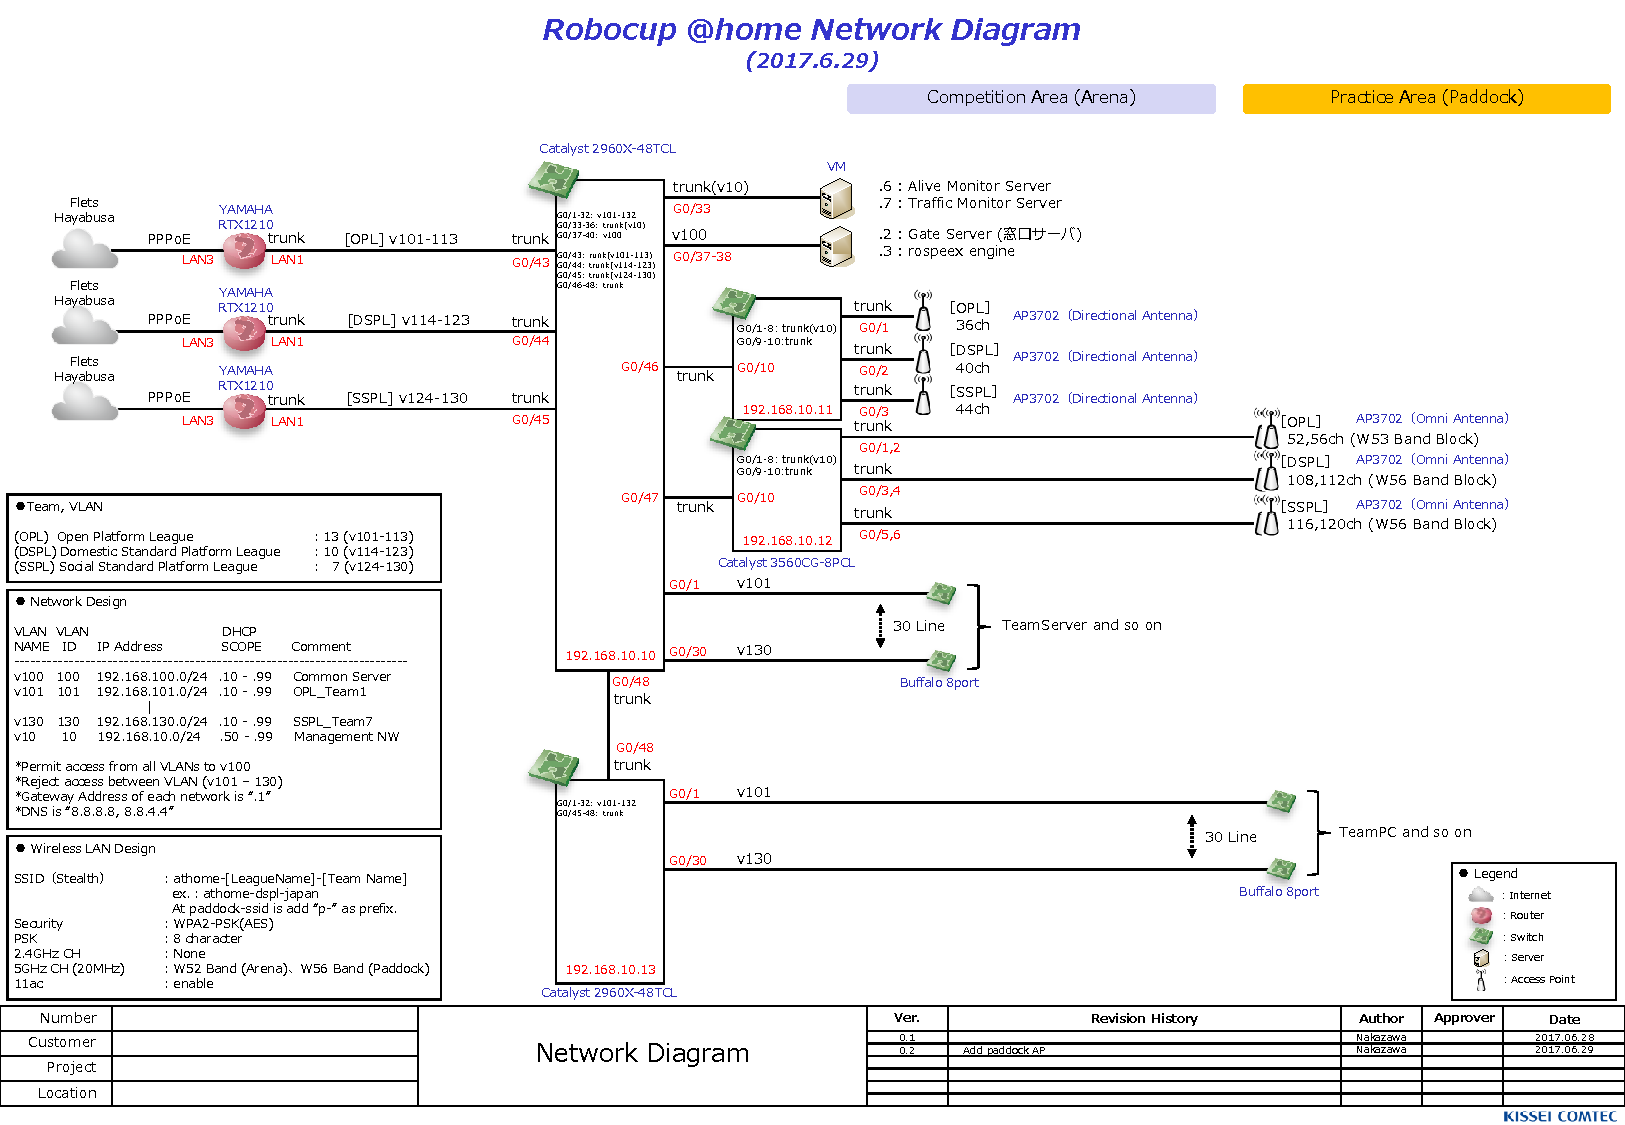
\includegraphics[rotate=90,width=\columnwidth]{images/nago2017_network.pdf}
	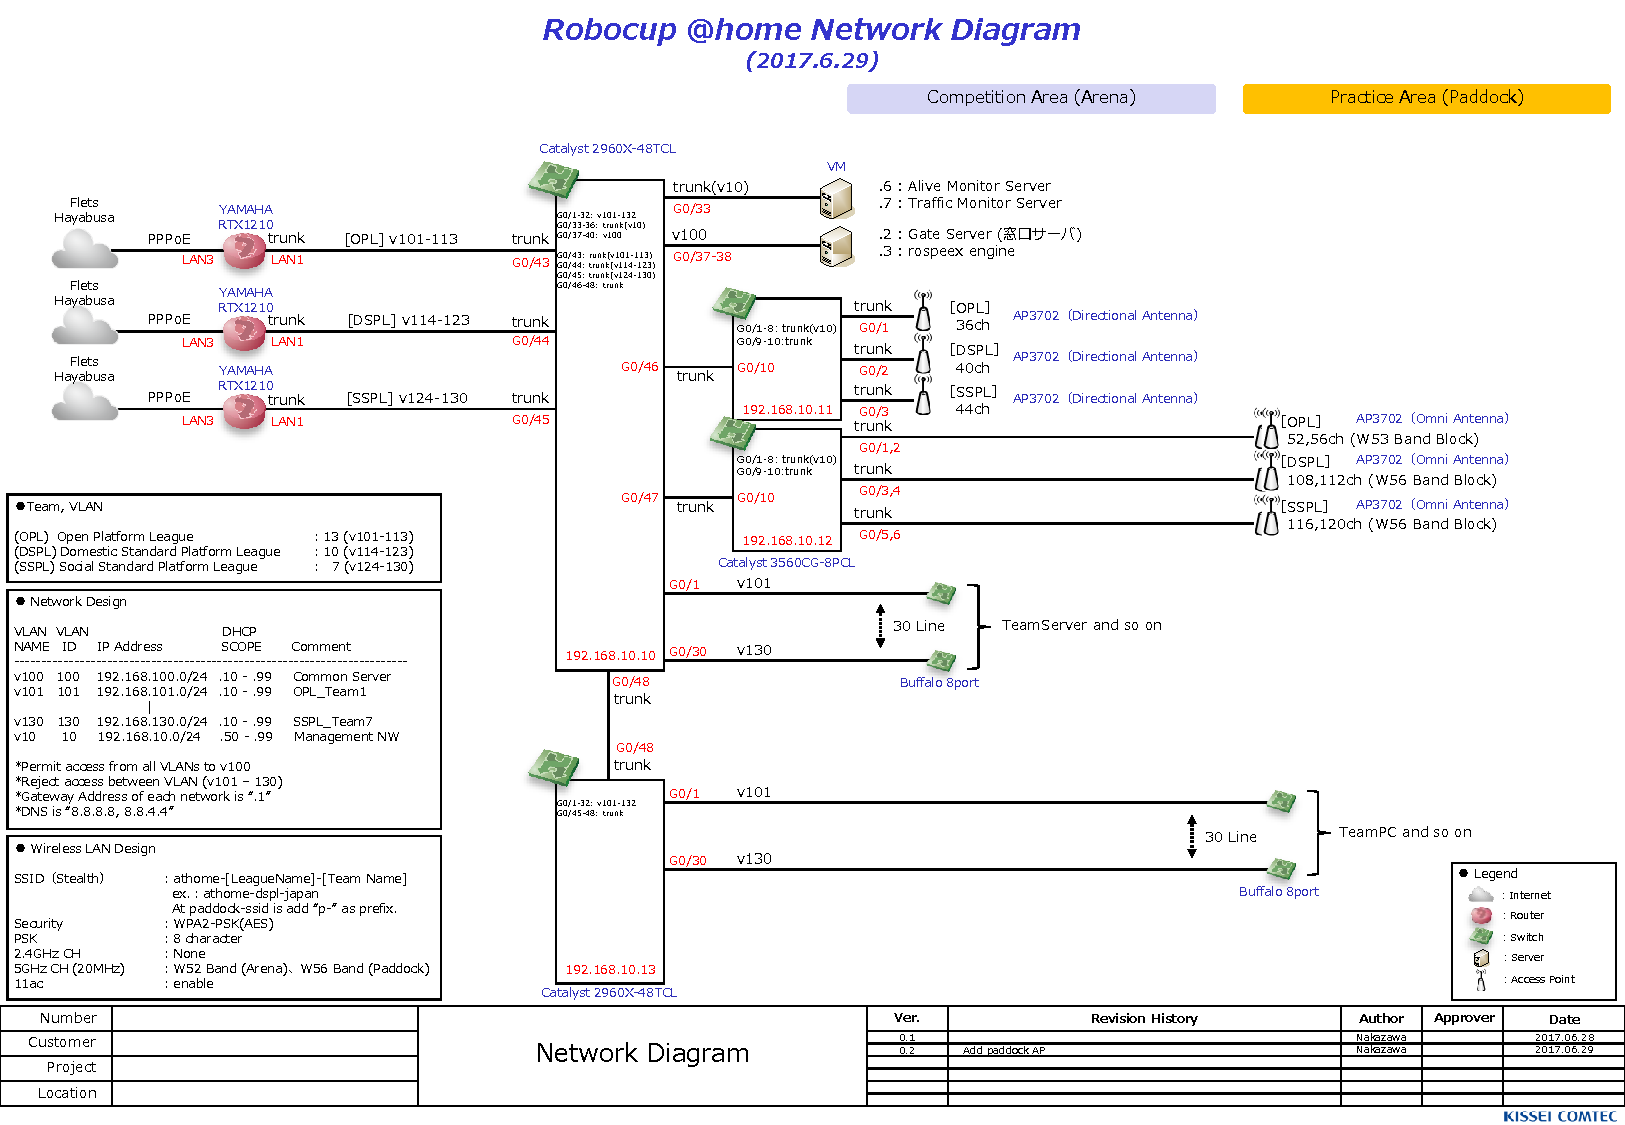
\includegraphics[width=\columnwidth]{images/nago2017_network.pdf}
\end{figure}

\end{itemize}
